\section{Geradlinige Dreiecks Darstellungen (SLTRs)}

Wie in der Einleitung schon geschrieben wurde wird sich diese Arbeit mit der Möglichkeit auseinandersetzten geradlinige Dreiecks Darstellungen für planare Graphen zu finden. Die nächste Definition formalisiert diese Darstellung, auf die wir im weiteren Verlauf der Arbeit immer wieder zurück kommen werden.

\begin{definition}[SLTR]\label{defsltr}
Eine Zeichnung eines planen Graphen $G$ wird \textit{geradlinige Dreiecksdarstellung}, im weiteren kurz \textit{SLTR} (für die englische Bezeichnung \textit{straight line triangle representation}), genannt falls gilt:
\begin{itemize}
\item[S1] Alle Kanten sind Segmente von Geraden.
\item[S2] Alle Gebiete, inklusive dem Äusseren, sind nicht degenerierte Dreiecke.
\end{itemize}
\end{definition}

\begin{figure}[h]
	\centering
  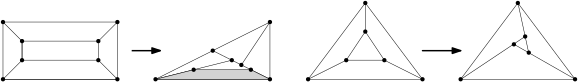
\includegraphics[width=0.8\textwidth]{sltr-example.png}
	\caption{Links einer der beiden 3-zusammenhängenden Graphen auf acht Knoten ohne SLTR und rechts ein Graph mit einer möglichen SLTR.}
\end{figure}

Für die weiteren Betrachtungen ist es nützlich drei Knoten $\{a_1,a_2,a_3\}$, die das äusseren Gebiet berühren, gesondert zu betrachten. Wir nennen sie die \textit{Aufhängungen} von $G$. $a_1,a_2$ und $a_3$ sind dann die designierten Ecken des äusseren Gebietes einer möglichen SLTR. Einen Graphen zusammen mit einem äusseren Gebiet und festen Aufhängungen als Paar zu behandeln ist sinnvoll, wie in Bespiel \ref{bsp1} zu sehen ist. Bevor wir zur ersten Proposition kommen wollen wir die Klasse der planaren Graphen, die wir betrachten etwas einschränken. Dabei hilft uns die nächste Definition.

\begin{definition}[intern-k-zusammenhängend]\label{int_3_con}
Ein Graph $G$ ist zusammenhängend falls für alle Knoten $u,v$ ein Pfad von $u$ nach $v$ exisitert. $G$ ist \textit{k-zusammenhängend}, falls er nach der Entfernung von $k-1$ beliebigen Knoten weiterhin zusammanhängend ist.\\
Sei $G$ plan mit den Aufhängungen $\{a_1,a_2,a_3\}$, weiter sei $a_\infty$ ein zusätzlicher Knoten eingefügt im äusseren Gebiet. Dann ist $G$ \textit{intern k-zusammenhängend}, falls $G+v_\infty\coloneqq(V\cup\{v_\infty \},E\cup \{(a_1,a_\infty),(a_2,a_\infty),(a_3,a_\infty)\})$ k-zusammenhängend ist. 
\end{definition}

Für intern-3-zusammenhängende planare Graphen ist die topologische Einbettung nach der Auswahl der Aufhängungen eindeutig (und somit auch die Menge der Gebiete $F$ von $G$). Die nächste Präposition enthält eine erste notwendige Bedingung für die Existenz von geradlinigen Dreiecksdarstellungen (SLTRs).

\begin{proposition}\cite[Proposition 1.2]{af13}
Sei $G$ ein planer Graph mit den Aufhängungen $\{a_1,a_2,a_3\}$ als äussere Ecken einer SLTR. Weiter gebe es keine inneren Knoten $v$ mit deg$(v) < 3$. Dann ist $G$ intern-3-zusammenhängend.
\end{proposition}

\begin{proof}
Sei $\Delta$ die SLTR von $G=(V,E)$. Angenommen es existiert eine Menge $U \subseteq V$ in $G$ mit $|U| = 2$, deren Entnahme $G$ in nicht zusammenhängende Komponenten trennt. Wir werden zeigen, dass jeder Teil von $G\backslash U$ eine der Aufhängungen enthält und somit $G + v_\infty$ nicht von $U$ getrennt wird. Jeder innerer Knoten in $G$ hat Grad grösser als zwei. Sei $K$ eine der Komponenten von $G\backslash U$, und sei $P$ ein Pfad der entsteht wenn wir $U$ wieder einfügen. Dann muss $K$ eine Aufhängung enthalten.

Falls $U$ keinen Pfad induziert, dann betrachte die konvexe Hülle von $U \cup K$ in $\Delta$. Mindestens drei der Ecken von $U \cup K$ haben Aussenwinkel grösser als $\pi$. Zwei dieser Winkel können an den Knoten aus $U$ liegen, aber der dritte muss ein Winkel sein der schon in $\Delta$ existiert. Es handelt sich somit um eine Aufhängung.
\end{proof}

\begin{remark}
Für innere Knoten von Grad 2 in einer SLTR müssen beide angrenzenden Winkel gerade sein. Somit kann man diese Knoten durch eine gerade Kante zwischen ihren Nachbarn ersetzen und den resultierenden Graphen betrachten. Wir werden somit von nun an nur intern-3-zusammenhängende Graphen mit Aufhängungen betrachten, da alle anderen Graphen, die eine SLTR zulassen, auf diese reduziert werden können.
\end{remark}

\begin{example}\label{bsp1}
Es existieren planare Graphen, von denen manche Einbettungen SLTRs zulassen, andere jedoch nicht. Betrachten wir den planaren Graphen mit zehn Knoten aus Abbildung \ref{10_example}. Mit rot und grün sind die beiden Gebiete markiert die jeweils einmal als das äussere Gebiet festgelegt wurden. Die topologische Einbettung auf der rechten Seite lässt zu dieser Wahl des äusseren Gebietes keine SLTR zu. Das nicht dreieckige Gebiet ist grau eingefärbt. Zu Auswahl auf der linken Seite existiert hingegen eine. Die Aufhängungen sind in beiden Fällen Eindeutig wegen $|f|=3$. Dies ist der kleinste 3-zusammenhängende kombinatorische Graph, der diese Eigenschaft hat.

\begin{figure}[h]
\centering
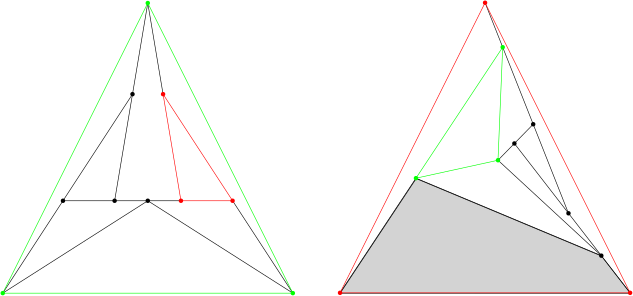
\includegraphics[width=0.7\textwidth]{10_example.png}
\caption{Zwei topologische Einbettungen des des (kombinatorisch) gleichen planaren Graphen, wobei die linke keine SLTR zulässt.}
\label{10_example}
\end{figure}

\end{example}

Zu den Fragen, welche notwendigen und hinreichenden Bedingungen für die Existenz von SLTRs gelten und welche algorithmischen Ansätze man bei der Suche nach einer spezifischen Darstellung verfolgen kann haben Aerts und Felsner einige Antworten geliefert. Die nächsten zwei Kapitel, werden sich mit diesen auseinandersetzen. Zuvor werden in diesem Kapitel noch einige Konzepte eingeführt, die notwendig sind um der Argumentation zu folgen.